\documentclass[a4paper, 12pt]{article}
\usepackage[american]{babel}
\usepackage[utf8]{inputenc}
\usepackage{csquotes}
\usepackage[style=apa,backend=biber,natbib=true]{biblatex}
\DeclareLanguageMapping{american}{american-apa}
\usepackage[T1]{fontenc}
\usepackage{mathptmx}
\usepackage{enumerate}
\usepackage{amsmath}
\usepackage{graphicx}
\usepackage{float}
\usepackage[margin=0.5in]{geometry}

\addbibresource{main.bib}

\renewcommand{\baselinestretch}{1.0}
\newcommand\nd{\textsuperscript{nd}\xspace}
\newcommand\rd{\textsuperscript{rd}\xspace}
\newcommand\nth{\textsuperscript{th}\xspace}

\graphicspath{{./figures/}}
\DeclareGraphicsExtensions{.pdf,.png,.jpeg}

\setlength\parindent{24pt}

% fill up your name, ID, contribution and paper title here
\author{
IZZMINHAL AKMAL BIN NORHISYAM \quad 242UC240JF \quad 25\% \\
CHOW YING TONG \quad 242UC244NK \quad 25\% \\
CHOONG JIA XUEN \quad 242UC244K1 \quad 25\% \\
LIM YU XUAN \quad 251UC18043 \quad 25\% \\
}
\title{ A Long-Term Probabilistic Forecast of AI-Driven E-Waste }

\begin{document}
\maketitle

\section*{Executive Summary}
In recent years, the rapid advancement of artificial intelligence (AI) has led to an unprecedented increase in computational demand, resulting in accelerated hardware obsolescence. This behaviour has led to a global AI-driven e-waste crisis that remains to be explored and covered by current research and inadequately addressed by the technology and electronics industry. Furthermore, the existing forecasting models like ones from \citet{wang_2024_ewaste} only accounts for e-waste until 2030, therefore creating a long-term forecasting gap. 
\par This research improves upon the Computational Power-driven Material Flow Analysis (CP-MFA) model to forecast AI-driven e-waste up to the year of 2035. In order to generate not just the baseline scenario, but also worst case and best case scenarios as a guide policymakers and industry leaders to curb the e-waste crisis, probabilistic modeling such as Monte Carlo simulations is used to capture real-world variability in hardware and operational factors.
\par The research methodologies used in this research builds upon the existing CP-MFA model with several key improvements, such as replacing the pre-existing exponential growth assumption with a sigmoid (S-curve) adoption model, accurately reflecting the market saturation and technological enhancements in the AI sector. In addition, a dynamic GPU power consumption model is utilised to account for workload fluctuations, hardware degradation and technological advancements in terms of hardware efficiency. Furthermore, \textbf{heterogeneous hardware modeling} is used to accurately reflect the refresh cycles of GPUs, CPUs and AI accelerators. A \textbf{circular economy feedback loop} and \textbf{regional infrastructure differentiation} highlights real-world electronics recycling rates, hardware reuse and material recovery as well as hardware deployment and lifespan in different geographical contexts. Finally, \textbf{probabilistic Monte Carlo simulations} are used to measure uncertainty and sensitivity in factors affecting e-waste forecasts, such as emissions from manufacturing, transport, and toxic waste disposal, which is part of the \textbf{lifecycle assessment}.
\par The expected outcome is to provide a long-term AI-driven e-waste forecast with confidence intervals, identifying the sensitive variables such as server lifespan, GPU efficiency and data center uptime that has the most influential impact on the forecast. This research will provide multiple scenario analysis and actionable insights for policymakers, industry leaders and researches to develop effective e-waste management strategies, and promote sustainable hardware practices. 
\par To aid policymakers, businesses and researches to accurately forecast and mitigate the environmental impacts of AI-related e-waste, this research aims to develop a close a significant research gap by providing a long-term forecast until 2035, through developing sustainable infrastructure, planning strategic policies, and raising awareness of the imminent e-waste crisis. \\

\textbf{Keywords:} Artificial Intelligence (AI), Electronic Waste (E-waste), Sustainability, Monte Carlo Simulation, Hardware Obsolescence

\section{Introduction}
The field of artificial intelligence (AI) is experiencing a major boom, best captured by the exponential growth in the computational resources required to train the latest, top-notch models. \citet{Sevilla_Roldan_2024} report that the amount of training compute increased by 4.4 times annually between February 2022 and May 2024. The widespread use of AI in companies across various industries is accompanied by an ever-increasing computational demand for training AI models. According to \citet{Maslej2025}, 78\% of businesses used AI in at least one business function, up from 55\% in 2023 (p.~262).

\par Modern AI's increased processing capacity depends on millions of physical servers that are driven by enormous data centers located all over the world.  These advanced infrastructures greatly increase the carbon footprint of the AI landscape, despite helping to enable training and powering the most recent AI models.  Embodied carbon, or the emissions released during the manufacturing of hardware components, accounts for the largest portion of AI's total carbon emissions, as noted by \citet{Wu2022} in their research (p.~5).

\par The end-of-life phase for the same hardware components is another factor that is often disregarded when assessing the carbon emissions of AI, aside from the manufacturing stage.  These days, hardware devices that are unable to meet the growing computational demands eventually lead to electronic waste, or "e-waste," particularly with the cycle of accelerated hardware obsolescence.

\section{Problem Statement}
\subsection*{The Root Problem}
The obsolescence of hardware that are no longer able to meet the computational demands of AI creates a global e-waste crisis, which is not adequately addressed by existing research and current industry practices. The scale of the problem, and the potential solutions to it are still unclear.

\subsection*{Research Gaps}
Through analyzing multiple research works, several research gaps can be identified: 
\begin{enumerate} 
	\item Lack of Long-Term E-Waste Forecasting: Although \citet{wang_2024_ewaste} present a foundational model that forecasts e-waste, its scope is limited to only the year 2030. Infrastructure policy planning and developing standard industry practices for dealing with obsolete devices are usually long-term efforts, a forecast that extends to at least 2035 is necessary. 
	
	\item Ethical and Regulatory Gaps: As highlighted by \citet{Zhuk2023}, there is an ethical and legal grey area when it comes to handling e-waste. The toxic components of e-waste from developed countries usually end up in the landfills of developing nations that do not have the capacity or recycling infrastructure to dispose of the e-waste properly. There is a need to revamp existing disposal policies to address this issue.
	
	\item Absence of Quantified Solutions: Although \citet{wang_2024_ewaste} found circular economy strategies for hardware devices to be useful in reducing e-waste by 58\%, the precise implementation methods for circular economy is unclear and not well-documented.
\end{enumerate}

\subsection*{Analysis and Comparison of Possible Research Problems}
Based on the research gaps identified, there are several research problems that arise: 

\begin{enumerate}
    \item The Strategic Planning Problem: Without accurate, long-term projections of AI-driven e-waste after 2030, governments and businesses are unable to make strategic, well-informed decisions regarding the development of sustainable hardware, the allocation of resources for waste management, and future recycling infrastructure. As a result, the world as a whole is not ready for the full impact of the e-waste wave that is expected to occur in the next ten to fifteen years.
 
	\item The Environmental Injustice Problem: The lack of clear international regulations and industry standards for the disposal of AI e-waste means that the harmful effects of the AI revolution are disproportionately felt by developing countries, which do not benefit in a significant way from the advancement of AI. Instead, they are now dealing with chronic soil contamination and other public health emergencies.
	
    \item The Implementation Issue: The AI sector is well aware of the concepts of circular economy. However, implementing it in the real world is quite challenging. This is because businesses are reluctant to invest in strategies like hardware lifespan extension or module reuse, due to the lack of reliable and accurate standardized models or metrics to confirm their economic viability. This inaction continues the linear "take-make-dispose" model, directly contributing to the growing e-waste crisis.
\end{enumerate}

Despite the enormous global significance of problem (2), solving the fundamental problems of international law and trade policy would necessitate a scope that goes well beyond this computer science research project.  Similarly, the highly proprietary nature of hardware life cycle data and the absence of standardized measurement models make investigating the possibility of a viable strategy for circular economy virtually impossible at the current moment, even though Problem (3) is crucial for the AI landscape.

\subsection*{Selection of A Research Problem}
After careful consideration, Problem (1) is selected as the main focus for this research proposal for the reasons as follows: 

\begin{itemize}
	\item Relevance and Significance: An essential first step is a forecast that lasts until at least 2035. It offers the information required to spur action on the other two issues. It is very hard to generate political will for new regulations (Problem 2) or encourage industry investment in innovative solutions (Problem 3) without a clear understanding of the actual scope of the upcoming crisis.
	
	\item Feasibility: This research can directly expand on the Computational Power-driven Material Flow Analysis (CP-MFA) model that Wang et al. (2024) have already proposed. With the methodology already in place, this research can concentrate on increasing its predictive capacity by adding fresh data and honing the hypotheses over a longer period of time.
	
	\item Measurable Outcome: A precise, quantifiable, and useful forecast will be the research's output.  Policymakers, business executives, and other researchers in the field will find this concrete outcome to be a useful contribution.
\end{itemize}

\section{Research Questions, Hypotheses and Objectives}
\subsection*{Research Questions}
\begin{enumerate}
	\item What is the projected volume and growth trajectory of AI-driven e-waste from 2030 to 2035 when modeling technology proliferation with a sigmoid (S-curve) adoption curve instead of an exponential one?
	\item How do key operational variables, such as server lifespan, GPU efficiency gains, and data center uptime contribute to the uncertainty and variability of long-term e-waste forecasts?
	\item To what extent can the accuracy of AI e-waste forecasting be improved by replacing deterministic assumptions with a probabilistic model that incorporates dynamic, real-world hardware parameters?
\end{enumerate}

\subsection*{Hypotheses}
\begin{enumerate}
	\item H1: The growth of AI-driven e-waste will decelerate post-2030, following a sigmoid pattern, but the cumulative volume by 2035 will significantly exceed linear extrapolations from earlier models.
	\item H2: A probabilistic forecast will reveal a wider and more realistic range of potential e-waste outcomes compared to a deterministic model, identifying server lifespan and GPU efficiency as the most sensitive parameters.
	\item H3: A dynamic forecasting model that accounts for workload-specific power consumption and heterogeneous hardware refresh cycles will produce significantly different and more accurate e-waste projections than a static, homogeneous model.
\end{enumerate}

\subsection*{Objectives}
\begin{enumerate}
	\item To develop an enhanced Computational Power-driven Material Flow Analysis (CP-MFA) model that extends e-waste projections to the year 2035.
	\item To evaluate the future risk by utilizing the probabilistic distributions for key hardware and operational parameters with the use of the Monte Carlo simulation framework.
	\item To provide policymakers and business executives with a useful tool by creating and evaluating a baseline, optimistic, and pessimistic e-waste projection for 2035.
\end{enumerate}

\section{Literature Review Summary}
Recent academics are having a discussion on artificial intelligence's effects on the environment that has evolved to focus more on AI's energy usage, bringing it to a more in-depth examination of the full hardware life cycle. \citet{Wu2022} showed that embodied carbon, defined as the emissions from producing AI hardware, makes up at least 50\% of AI's overall carbon footprint (p.~5). This perspective emphasizes the importance of considering the entire life cycle for all hardware components, from manufacturing to eventual disposal as electronic waste (e-waste). The sustainability of AI applications in any industry is linked to the environmental costs of the underlying hardware infrastructure, as further evidenced by research by \citet{M.rauf2024} on AI's role in electric vehicles.

 In the recent studies, they have started to notice the growing e-waste crisis is significantly increased due to the AI industry's rapid hardware obsolescence. \citet{wang_2024_ewaste} made a very important contribution in this field by creating the first Computational Power-driven Material Flow Analysis (CP-MFA) model. This model proposes a quantitative framework for predicting the amount of e-waste produced by AI servers. Without any question, the CP-MFA is a huge achievement in the research. However, because the scope is only limited to 2030, this creates a huge gap in the literature. This is due to the fact that waste management planning and working policies require far more strategic foresight. 

The study from \citet{Zhuk2023} highlights the environmental injustice of shipping dangerous e-waste to all those countries that lack facilities and proper equipment to dispose of all the e-waste properly. These countries often couldn't manage the e-waste, and it is extremely challenging to create the political will required to enact and enforce the strong international regulations that Zhuk argues are required in the absence of a reliable, long-term forecast that fully measures and quantifies the scale of the upcoming e-waste wave.

\section{Research Methodology}
This study employs a dynamic, probabilistic modeling approach to analyze the electronic waste (E-waste) generated by generative artificial intelligence (GAI) infrastructure, specifically AI servers supporting large language models (LLMs). Building on the Computational Power-driven Material Flow Analysis (CP-MFA) framework introduced by Wang et al. (2024), the methodology incorporates several improvements to realistically represent hardware lifecycle, operational factors, technology adoption, and circular economy impacts.

\subsection{Model Structure}
The core of the model predicts quarterly global deployments, in-use stocks, and end-of-service (EoS) E-waste from AI servers from 2020 to 2035. The computational power demand is linked to a benchmark GPU server (8-unit Nvidia DGX H100 system) to convert computational requirements into physical hardware stock and waste. Unlike prior exponential growth assumptions, this method applies a sigmoid adoption curve reflecting training-data-size constraints and technology maturation.

\subsection{Key Parameterization}
The model parameters are informed by empirical data and literature:

\begin{enumerate}
    \item Server Lifespan: Modeled as a normal distribution with a mean of 3.5 years and standard deviation of 0.8 years, reflecting industry data for compute hardware lifespans \citep{wang_2024_ewaste}.
    \item GPU Efficiency Gains: Represented by a uniform distribution between 15\% and 40\% efficiency improvement per generation, informed by Nvidia GPU power management studies showing generation-over-generation reductions in power use \citep{nvidia-2023, you-2023}.
    \item Data Center Uptime: Modeled as a Beta distribution with shape parameters $\alpha=17$ and $\beta=1.5$, ranging from 85\% to 98\%, capturing realistic enterprise data center operational uptimes across Tier 1 to Tier 4 facilities \citep{unknown-author-no-date, operations-2024}.
    \item User Adoption Rates: Follow a log-normal distribution consistent with technology diffusion literature and sigmoid S-curve adoption behavior observed in AI deployments \citep{operations-2024, pamplona-2024}.
    \item Market Penetration Caps: Triangular distribution with minimum 60\%, mode 80\%, and maximum 95\%, capturing saturation and market maturity levels derived from technology adoption frameworks \citep{fordyce-2025}.
    \item Hardware Failure Rates: Beta distribution ranging 2\%-8\% annually, based on reported failure rates of GPUs and server components in operational data centers \citep{wang_2024_ewaste}.
    \item Utilization Rates: Normal distribution with mean 70\% and standard deviation 15\%, truncated between 40\% and 90\%, consistent with reported server workload levels \citep{wang_2024_ewaste}.
    \item Regional Deployment Timing: Applied as a normal distribution with ±6 months variation to model geographic variability in AI infrastructure rollouts.
    \item Upgrade Thresholds: Uniform distribution spanning 20\%-40\% performance degradation due to factors like thermal throttling and aging hardware, motivating hardware refresh decisions \citep{you-2023}.
    \item Recycling Success Rates: Beta distribution with 70\%-95\% material recovery rates, based on current e-waste recycling performance worldwide \citep{wang_2024_ewaste}.
\end{enumerate}

\subsection{Methodological Enhancements}
\subsubsection{Dynamic GPU Power Consumption Modeling}
Modern AI hardware exhibits significant variability in power consumption over time due to workload demands, thermal management, and architectural improvements. Instead of assuming constant computational power intensity per GPU server, the model integrates dynamic power consumption curves that capture real-world variations. Empirical studies from Nvidia GPU power management demonstrate generation-over-generation power efficiency gains ranging from 15\% to 40\%, achieved through advanced power sharing, dynamic voltage and frequency scaling (DVFS), and task-specific optimization. The model also accounts for thermal throttling and gradual performance degradation over the lifespan of GPUs, which typically triggers upgrades once performance drops between 20\% to 40\%. Incorporating these time-varying and hardware-specific behaviors enhances the accuracy of power usage estimation and aligns e-waste projections with observed operational realities in AI data centers \citep{you-2023, nvidia-2023, wang_2024_ewaste}.

\subsubsection{Data Center Uptime Integration}
Operational uptime in data centers is never absolute; factors like scheduled maintenance, unexpected outages, and load balancing create realistic periods of server inactivity or reduced utilization. The model applies a Beta distribution to represent enterprise data center uptime percentages, spanning 85\% to 98\%, reflecting the diversity from Tier 1 to Tier 4 facility standards. This integration adjusts server utilization rates downward from naive 100\% assumptions, realistically reflecting operational availability that impacts effective computational capacity and hardware wear. Such nuanced uptime modeling ensures that the estimation of deployed server stock and resulting e-waste properly considers real operational environments and maintenance cycles, ultimately leading to more precise forecasting of EoS hardware volumes \citep{unknown-author-no-date, operations-2024, wang_2024_ewaste}.

\subsubsection{Sigmoid Technology Adoption Curve}
Classical models rely on exponential computational growth via Moore’s Law, which simplifies technology proliferation estimates but fails to accommodate the real-world saturation effects of market limits and technology maturation. This method replaces exponential growth with a sigmoid or S-curve adoption trajectory that captures the initial slow uptake, rapid mid-phase expansion, and eventual plateauing as the market saturates the addressable user base and computational demands stabilize. The log-normal distribution fits historical technology adoption patterns and reflects variability in global AI infrastructure deployments. Embracing sigmoid growth constraints tied to a finite training data set and realistic adoption limits generates plausible scenarios for GAI proliferation and associated e-waste flows more consistent with observed technology diffusion dynamics \citep{pamplona-2024, fordyce-2025, wang_2024_ewaste}.

\subsubsection{Heterogeneous Hardware Modeling}
Data centers deploy a mixed inventory of server hardware encompassing varying generations of GPUs, CPUs, and emergent AI accelerators like TPUs or custom ASICs. The enhanced model captures this heterogeneity by representing servers with differing performance and power profiles and modeling staggered, non-uniform hardware refresh cycles. For example, GPU upgrades often occur approximately every two years, aligning with commercial release and deprecation schedules. This approach departs from simplified uniform-replacement assumptions to reflect realistic operational practices, including partial fleet refresh and maintenance-driven incremental updates. Explicitly modeling heterogeneity enables more accurate estimates of material flows, component-specific e-waste, and the effects of specialized AI hardware beyond traditional GPUs \citep{wang_2024_ewaste}.

\subsubsection{Workload-Specific Power Modeling}
AI workloads are diverse in nature and computational intensity depending on the task, such as training versus inference or domain-specific models like NLP and computer vision. This methodology differentiates power consumption profiles based on workload type and stage, incorporating reductions from efficient model compression, pruning, and optimization techniques that alleviate hardware demands without sacrificing accuracy. By integrating workload-level variability, this modeling avoids one-size-fits-all power assumptions, thus enhancing granularity for environmental impact analysis and forecasting the energy and e-waste implications of evolving AI applications and optimizations \citep{wang_2024_ewaste, you-2023}.

\subsubsection{Circular Economy Feedback Loops}
The model explicitly incorporates circular economy principles by simulating how recycling success rates (modeled as a Beta distribution from 70\% to 95\%) affect the demand for new hardware, closing the loop between materials recovered from end-of-life servers and newly manufactured components. It also accounts for geopolitical supply chain constraints, including rare earth element availability and trade-based technical barriers affecting component sourcing and regional deployment. Strategies such as lifespan extension through improved maintenance, module reuse by dismantling and repurposing critical components, and stepwise upgrading are modeled as they demonstrably reduce net e-waste generation. These feedback mechanisms imbue the model with strategic insight into how circular processes can mitigate e-waste growth amid the GAI boom \citep{wang_2024_ewaste}.

\subsubsection{Probabilistic Scenario Analysis}
To address uncertainty inherent in parameters like hardware failure rates, utilization, and adoption speeds, the enhanced methodology replaces deterministic scenario evaluation with Monte Carlo simulations using empirically grounded parameter distributions (e.g., Normal, Beta, Triangular). This probabilistic approach yields confidence intervals, revealing the range of possible e-waste outcomes and identifying sensitivities and risks. By embracing stochastic variability through repeated sampling, the model offers robust foresight for decision-making and policy formulation under uncertainty, improving upon previous single-value point estimates \citep{wang_2024_ewaste}.

\subsubsection{Regional Infrastructure Variations}
Recognizing geographic heterogeneity, the model incorporates differential regional standards in data center efficiency, hardware lifespans affected by climate and usage patterns, and variability in recycling infrastructure and regulatory environments. Server deployment proportions are modeled across major clusters—North America, East Asia, and Europe—with ±6 months timing variation to reflect logistic and supply chain disparities. This spatial differentiation is critical to accurately representing global e-waste flows and identifying region-specific challenges and interventions \citep{wang_2024_ewaste}.

\subsubsection{Lifecycle Assessment Enhancement}
Extending beyond servers, the methodology includes networking equipment, storage arrays, and cooling infrastructure in the lifecycle inventory, modeling component-level replacement patterns such as discrete GPU swaps versus full server decommissioning. Emissions from manufacturing and transportation phases and toxic material releases (lead, chromium, cadmium) from e-waste are integrated, augmenting environmental impact assessments. Economic valuation of recovered materials (\~\$70 billion potential globally) and environmental benefits of recycling are quantified, thus providing a holistic lifecycle perspective bridging physical material flows and sustainability outcomes \citep{wang_2024_ewaste}.

\section{Research Activities and Milestones}

The activities and milestones can be separated into multiple phases:

\begin{enumerate}
    \item \textbf{Data Collection \& Model Foundation}
    \begin{enumerate}
        \item Complete GPU performance data collection
        \item Establish data center partnerships for operational metrics
        \item \textbf{Milestone:} GPU power consumption database compiled
        \item Gather GAI adoption statistics and historical trends
        \item Collect regional infrastructure data
        \item \textbf{Milestone:} Comprehensive dataset assembled
        \item Develop dynamic GPU power consumption curves
        \item Build sigmoid technology adoption models
        \item \textbf{Milestone:} Core modeling components ready
    \end{enumerate}
    
    \item \textbf{Framework Development}
    \begin{enumerate}
        \item Implement CP-MFA framework with heterogeneous hardware modeling
        \item Define Monte Carlo parameter distributions
        \item \textbf{Milestone:} Base simulation framework operational
        \item Integrate workload-specific power modeling
        \item Add circular economy feedback loops
        \item \textbf{Milestone:} Enhanced model features implemented
        \item Complete lifecycle assessment expansion
        \item Finalize regional infrastructure variations
        \item \textbf{Milestone:} Full methodology framework complete
    \end{enumerate}
    
    \item \textbf{Simulation \& Analysis}
    \begin{enumerate}
        \item Execute Monte Carlo simulations (10,000 iterations)
        \item Initial statistical analysis of outputs
        \item \textbf{Milestone:} Simulation results generated
        \item Perform comprehensive sensitivity analysis
        \item Calculate confidence intervals and risk assessments
        \item \textbf{Milestone:} Statistical analysis complete
        \item Results interpretation and scenario comparison
        \item Validation against existing data
        \item \textbf{Milestone:} Analysis findings finalized
    \end{enumerate}
    
    \item \textbf{Dissemination}
    \begin{enumerate}
        \item Draft research paper and policy recommendations
        \item Prepare industry guidelines
        \item \textbf{Milestone:} Initial manuscript complete
        \item Peer review process and revisions
        \item Stakeholder consultations
        \item \textbf{Milestone:} Revised manuscript ready
        \item Final publication submission
        \item Conference presentations and dissemination
        \item \textbf{Milestone:} Research published and disseminated
    \end{enumerate}
\end{enumerate}

\subsection{Research Activities Flowchart}

\begin{figure}[H]
    \begin{center}
        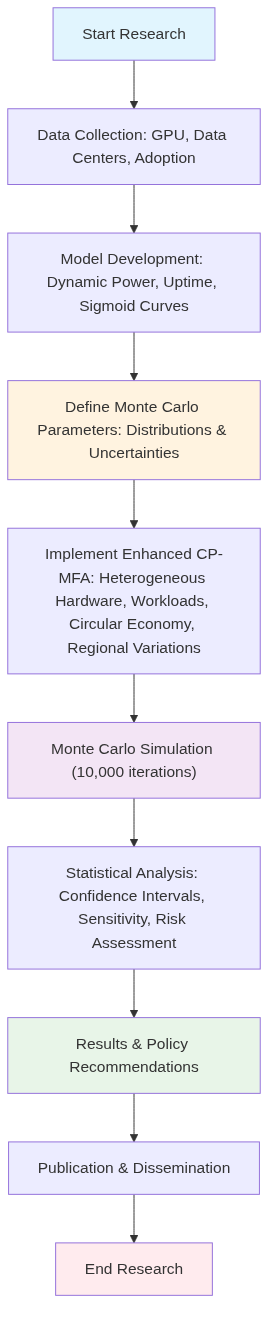
\includegraphics[width=0.2\textwidth]{flowchart}
    \end{center}
    \caption{Flowchart of the research activities}\label{fig:flowchart}
\end{figure}

\begin{figure}[H]
    \begin{center}
        \includegraphics[width=1.0\textwidth]{gantt_chart}
    \end{center}
    \caption{Gantt chart of the research milestones}\label{fig:gantt_chart}
\end{figure}

\section{Expected Results and Impact}
By providing actionable evidence for governments, regulators and industry leaders to design long-term e-waste management policies and practices, extending beyond 2030, this research will equip data center operators, AI companies and hardware manufacturers to plan sustainable hardware lifecycles and investments in circular economy practices. Through highlighting the gap in recycling infrastructures in developed and developing regions, this research serves as a guide to reducing the carbon footprint and toxic waste burden in different geographic backgrounds by identifying hardware recycling, reuse, and efficiency improvements. Finally, in hopes to aid stakeholders to anticipate future AI-related sustainability challenges, preparing infrastructure and regulations to properly confront the forecasted 2035 e-waste crisis, this research enhances models used for e-waste forecasting through probabilistic simulations, heterogeneous hardware modeling, and lifecycle integration.

%References
\printbibliography

\end{document}

